\subsection{Widersprüche der Anforderungen}\label{subsec:widersprueche}
\gqq{Zwei Anforderungen widersprechen einander, wenn sie nicht durch dieselbe technische Lösung umgesetzt werden können.}\autocite[][S.233]{Herrmann.2022}
So definiert Herrmann Widersprüche.
Widersprüche können sich aus unterschiedlichen Gründen ergeben.
So können Widersprüche zum Beispiel in Bezug auf die Qualität, die Kosten oder die Zeit entstehen.

In diesem Kapitel wird erläutert, wie Widersprüche erkannt, analysiert und gelöst werden können.

\subsubsection{Erkennen von Widersprüchen}\label{subsubsec:erkennung}
Bevor Widersprüche gelöst werden können, müssen sie zuerst erkannt werden.
Es gibt verschiedene Indikatoren, die auf Widersprüche hinweisen können.
\begin{itemize}
    \item Bisher getroffene Aussagen werden ignoriert oder verändert, so als wären diese nie getroffen worden.
    \item Blindes Zustimmen zu oder Ablehnen von Aussagen anderer.
    \item Pedanterie
    \item Aussagen anderer werden bis ins kleinste Detail hinterfragt.
    \item Informationen oder Informationsdetails werden verheimlicht.
    \item Man lässt sich nur auf vage Aussagen ein, mit der Aufforderung an andere, diese zu detaillieren.
\end{itemize}~\autocite[vgl.][S.43]{OliverCreighton.2012}

\subsubsection{Analyse von Widersprüchen}\label{subsubsec:analyse}
Bevor Widersprüche gelöst werden können, müssen diese analysiert werden.
Dazu werden die Ursachen für den Widerspruch ermittelt.
Auch können Widersprüche in verschiedene Kategorien eingeteilt werden.

Hierbei wird zwischen drei~\nameref{subsection:widerspruchsarten} unterschieden:
\begin{itemize}
    \item Inkonsistenz
    \item Anforderungskonflikte
    \item Machbarkeitskonflikte
\end{itemize}~\autocite[vgl.][S.235f]{OliverCreighton.2012}

\subsubsection{Lösen von Widersprüchen}\label{subsubsec:loesen}
Alle Widersprüche auf einmal zu lösen, ist nicht möglich,
denn durch das Lösen eines Widerspruchs kann ein anderer entstehen.
Daher ist es wichtig, die Widersprüche in einer bestimmten Reihenfolge zu lösen.
Hierbei wird sich zuerst auf Widersprüche auf höchster und abstraktester Ebene konzentriert,
denn diese haben die größte Auswirkung auf das System und arbeitet sich dann nach unten vor.

\paragraph{Reihenfolge der Widerspruchsauflösung}
\begin{enumerate}
    \item Durch ein Anforderungsreview Inkonsistenzen und Anforderungskonflikte erkennen.
    \item Inkonsistenzen im Problemraum lösen.
    \item Konflikte zwischen Stakeholder lösen.
    \item Anforderungskonflikte und Machbarkeitskonflikte im Lösungsraum lösen.
    Hier kommen zum Beispiel Nutzwertanalysen oder Quality Function Deployment zum Einsatz.
\end{enumerate}\autocite[vgl.][S.237f]{Herrmann.2022}

\subsubsection{Konflikttypen}
Um Konflikte besser lösen zu können, ist es wichtig, die verschiedenen Konflikttypen zu kennen.
Diese sind:
\begin{itemize}
    \item Sachkonflikt
    \item Datenkonflikt
    \item Interessenkonflikt
    \item Wertekonflikt
    \item Beziehungskonflikt
    \item Struktureller Konflikt
\end{itemize}\autocite[vgl.][S.137]{Pohl.2021}

\paragraph{Sachkonflikt}
\gqq{
    Ein Sachkonflikt zwischen zwei oder mehr Stakeholdern ist durch einen Mangel an Informationen
    oder durch Fehlinformation gekennzeichnet.
}~\autocite[][S.138]{Pohl.2021}

\paragraph{Datenkonflikt}
\gqq{
    Eine spezielle Ausprägung des Sachkonflikts ist der Datenkonflikt (auch Benennungskonflikt).
    Bei einem Datenkonflikt verstehen die beteiligten Stakeholder unterschiedliche Dinge unter einem Bezeichner.
}~\autocite[][S.138]{Pohl.2021}

\paragraph{Interessenkonflikt}
\gqq{
    Ein Interessenkonflikt zwischen zwei oder mehr Stakeholdern ist durch
    subjektiv oder objektiv verschiedene Interessen oder Ziele der Stakeholder gekennzeichnet.
}~\autocite[][S.138]{Pohl.2021}

\paragraph{Wertekonflikt}
\gqq{
    Ein Wertekonflikt ist durch verschiedene Kriterien (z. B. kulturelle Unterschiede, persönliche Ideale)
    von Stakeholdern zur Bewertung von Sachverhalten gekennzeichnet.
}~\autocite[][S.138]{Pohl.2021}

\paragraph{Beziehungskonflikt}
\gqq{
    Ein Beziehungskonflikt ist durch starke Emotionen, stereotype Beziehungskonzepte, schlechte Kommunikation
    oder negatives zwischenmenschliches Verhalten von Stakeholdern untereinander
    (z. B. Missachtung, Beleidigung) gekennzeichnet.
}~\autocite[][S.138]{Pohl.2021}

\paragraph{Struktureller Konflikt}
\gqq{
    Ein struktureller Konflikt ist durch ungleiche Macht- und Autoritätsverhältnisse
    zwischen Stakeholdern gekennzeichnet.
}~\autocite[][S.138]{Pohl.2021}

\subsubsection{Konsolidierungstechniken}
Es gibt verschiedene Konfliktlösungstechniken,
die bei der Konsolidierung von Widersprüchen helfen können.
Die Lösungstechniken werden in der Regel in der genannten Reihenfolge angewendet.
Diese sind:
\begin{enumerate}
    \item Einigung
    \item Kompromiss
    \item Abstimmung
    \item Variantenbildung
    \item Ober-sticht-Unter
\end{enumerate}\autocite[vgl.][S.139]{Pohl.2021}

\paragraph{Einigung}
\gqq{
    Bei der Konfliktlösungstechnik Einigung handeln die Konfliktparteien eine Lösung des Konflikts aus.
    Die Konfliktparteien tauschen Informationen, Argumente und Meinungen aus
    und versuchen sich gegenseitig im Dialog von der Richtigkeit des eigenen Standpunkts zu überzeugen
    und sich so auf eine Lösungsalternative des Konflikts zu einigen.
}~\autocite[][S.139]{Pohl.2021}

\paragraph{Kompromiss}
\gqq{
    Bei der Konfliktlösungstechnik Kompromiss versuchen die Konfliktparteien im Rahmen einer Diskussion
    einen Kompromiss zwischen den verfügbaren Lösungsalternativen zu finden.
    Im Unterschied zur Einigung besteht ein Kompromiss aus einer Kombination
    von Teilen der verfügbaren Lösungsalternativen.
    Ebenso kann ein Kompromiss auch darin bestehen,
    dass alle Lösungsalternativen verworfen werden und eine vollkommen neue und kreative Lösung entwickelt wird.
}~\autocite[][S.140]{Pohl.2021}

\paragraph{Abstimmung}
\gqq{
    Bei der Konfliktlösungstechnik Abstimmung wird die Lösung eines Konflikts durch eine Abstimmung erzielt.
    Die zur Wahl stehenden Alternativen werden den relevanten Stakeholdern zur Abstimmung vorgelegt.
    Jeder Stakeholder gibt seine Stimme einer der Alternativen.
    Die Alternative mit den meisten Stimmen wird als Konfliktlösung festgehalten.
}~\autocite[][S.140]{Pohl.2021}

\paragraph{Variantenbildung}
\gqq{
    Bei der Konfliktlösungstechnik Variantenbildung wird das System so gestaltet,
    dass durch Variantenauswahl oder Parametrierung verschiedene Systemvarianten realisiert
    oder Auswahlmöglichkeiten bei variablen Systemmerkmalen ermöglicht werden,
    wodurch das System unterschiedlichen, im Konflikt stehenden Interessen von Stakeholdern genügen kann.
}~\autocite[][S.140]{Pohl.2021}

\paragraph{Ober-sticht-Unter}
\gqq{
    Bei der Konfliktlösungstechnik Ober-sticht-Unter wird ein Konflikt anhand der Hierarchie
    der Konfliktparteien entschieden, d.h., die Konfliktpartei mit dem höheren organisatorischen Rang
    gewinnt den Konflikt.
    Wenn beide Konfliktparteien den gleichen organisatorischen Rang einnehmen,
    wird der Konflikt durch eine übergeordnete Instanz (z.B. einen Vorgesetzten) entschieden.
    Diese Konfliktlösungstechnik ist nur dann empfehlenswert,
    wenn andere Lösungstechniken zu keiner Lösung geführt haben (z.B. kein Kompromiss gefunden werden konnte)
    oder aus Ressourcengründen nicht anwendbar sind.
}


In Abbildung~\nameref{fig:konsolidierungstechniken} ist eine Übersicht über die Konsolidierungstechniken dargestellt,
und wann es sinnvoll ist diese anzuwenden.
\begin{figure}[ht]
    \centering
    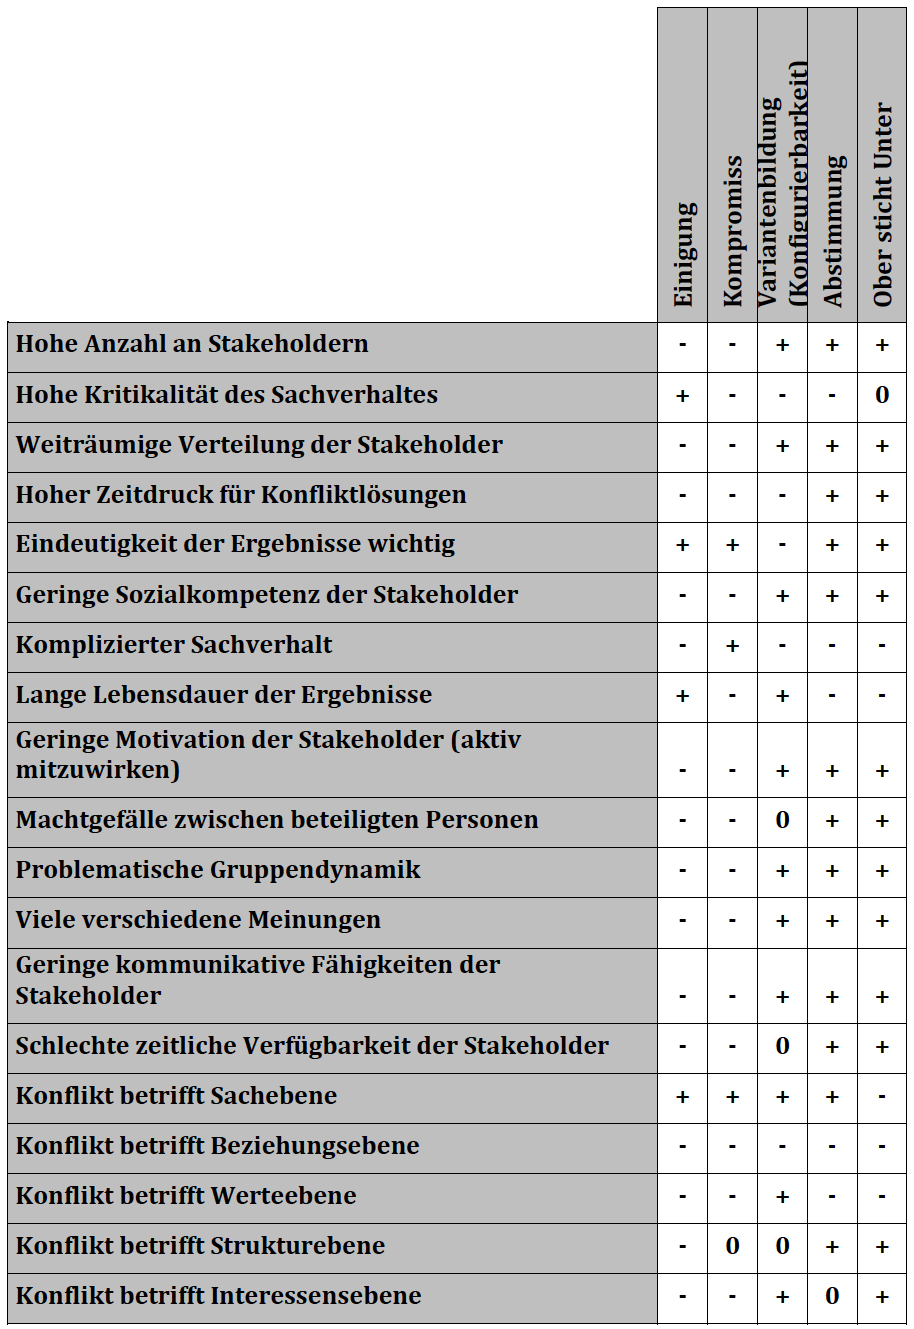
\includegraphics[width=0.8\textwidth]{images/KonsolidierungstechnikenTabelle}
    \caption{Konsolidierungstechniken}
    \label{fig:konsolidierungstechniken}
\end{figure}~\autocite[Abbildung 5][S.45]{OliverCreighton.2012}